\documentclass{article}

\usepackage{wrapfig}
\usepackage[colorlinks=true]{hyperref}
\usepackage{graphicx}
\usepackage{listings}
\usepackage[utf8]{inputenc}

\author{
	Alexander Faithfull\\IT University of Copenhagen\\\texttt{alef@itu.dk}
	\and
	Jesper Bengtson\\IT University of Copenhagen\\\texttt{jebe@itu.dk}}
\title{Coqoon: towards a\\modern IDE for Coq}

\date{}

\begin{document}

\maketitle

\noindent
Users of modern IDEs expect sophisticated features like automatic dependency
resolution, background recompilation, content-aware search features (such as
``show me where this is defined''), automatic indentation, syntax highlighting
and code completion. Coqoon, which is built on top of the Eclipse platform,
provides such an IDE for Coq.

Coqoon has two design goals. The first of these is to provide a
state-of-the-art Coq IDE; the second, more important, goal is to provide
reusable components to make it possible to embed support for Coq into other
Eclipse projects. For example, Coqoon was originally developed as part of
Kopitiam~\cite{DBLP:conf/nfm/Mehnert11}, a verification environment for Java
programs, and has now become the foundation upon which Kopitiam builds: the
abstraction layer between Coq and Eclipse.

Ultimately, we seek to provide a complete development environment for verified
Java programs. Developers will design models for programs in Coq using
separation logic before using these models to annotate Java programs with
their own specifications. A Coq-driven back end will then make it possible for
them to step through these annotated Java programs as though they were Coq
proofs, watching how the program state changes after each statement---and, when
necessary, inserting extra Coq commands to allow symbolic execution to proceed.
Coqoon will provide both a necessary part of the UI for this vision and the
glue that makes the interaction work behind the scenes.

\paragraph{Architecture and installation}

Coqoon is implemented as a pair of plug-ins for the Eclipse platform. One
implements the \emph{ideslave} communications protocol used to communicate
with recent versions of Coq, a model for managing Coq projects and
proof scripts, and a builder for automatically recompiling proof scripts when
their dependencies change. The other provides a user interface to that
functionality, including a CoqIde/Proof General-like editor for Coq
proof scripts.

\pagebreak

\begin{wrapfigure}{R}{0.23\textwidth}
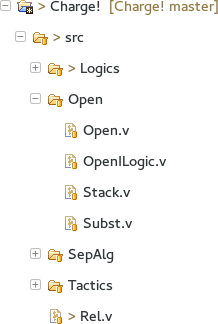
\includegraphics[width=0.23\textwidth]{project}
\end{wrapfigure}
The most user-visible consequence of installing these plug-ins is the support
for Coq projects \emph{(see right)}. This brings Java-like project management
to the Coq world: projects automate the processes of compiling source files and
configuring load paths.

Coqoon can be added to any installation of a recent version of Eclipse, and it
interoperates well with other plug-ins: for example, Java projects can contain
complete Coq developments, and Coq projects can be managed by the many version
control systems supported by Eclipse.

\paragraph{The model}

The Coq model is the core of Coqoon. Inspired by Eclipse's model for Java code,
it transforms basic Eclipse concepts into more structured Coq ones: for
example, an Eclipse text document can be presented as an organised hierarchy of
Coq sentences, sections and theorems. The model frees Coqoon---and software
built on top of it, like Kopitiam---from the need to repeatedly reimplement
low-level details, like lexing and parsing proof scripts, instead allowing them
to operate directly on higher-level Coq concepts.

\paragraph{Building projects}

Coqoon doesn't use \texttt{coqdep} or \texttt{coq\_makefile}; it instead
implements its own, more portable, build system. This system, triggered
whenever files in a Coq project are changed, automatically analyses Coq proof
scripts and their interdependencies before recompiling them as appropriate.

The Coqoon build system behaves like Eclipse's own Java build system: that is,
a proof script at \texttt{src/Example/Namespace/Basic.v} will be compiled into
the library \texttt{bin/Example/Namespace/Basics.vo}, which will have the
fully-qualified name \texttt{Example.Namespace.Basics}.

The Coqoon project builder also produces a project-specific \texttt{Makefile}
which implements a similar build system, including the separation between
source and binary hierarchies, to make it easy to work on Coqoon projects
without using Coqoon.

\paragraph{Conclusion}

Coqoon offers a new way to interact with Coq---one which offers useful new
functionality to long-time users, lowers the barriers to entry for beginners,
and makes it possible for developers to integrate Coq support into their own
tools.

More information about Coqoon, including installation instructions and links to
both precompiled Eclipse plugins and the source code, is available from
\linebreak
\url{http://www.itu.dk/research/tomeso/coqoon/}.

\bibliographystyle{plain}
\bibliography{coq6}

\end{document}
